\documentclass[11pt,a4paper]{article}
\usepackage{times,latexsym}
\usepackage[T1]{fontenc}
\usepackage{url}
\usepackage{booktabs}
\usepackage{amsmath,amssymb}
\usepackage{graphicx}
\usepackage{microtype}
\makeatletter
\def\input@path{{tacl-style/}}
\makeatother
\usepackage[acceptedWithA]{tacl2021v1}

\title{Provenance-Constrained Selective Language Style Planning from Sparse Evidence}

\author{Jiang Luchang\\
\texttt{auroral.sunflower@gmail.com}\\
\url{https://orcid.org/0009-0004-4579-4243}}
\date{Zenodo preprint | Version 1.0 | 25 August 2026}

\newcommand{\system}{\textsc{PersonaVoice}}
\hypersetup{
  pdftitle={Provenance-Constrained Selective Language Style Planning from Sparse Evidence},
  pdfauthor={Jiang Luchang},
  pdfsubject={Zenodo preprint},
  pdfkeywords={selective prediction, provenance, citation, language style, abstention, voice safety}
}
\begin{document}
\maketitle

\begin{abstract}
Memorial voice systems pose a language-generation problem before they pose a
  speech-synthesis problem: a system may have only a few historical messages and
  conflicting recollections, yet fluent output can be mistaken for words or
  beliefs that a person actually expressed.  We formulate
  \emph{provenance-constrained language style planning}, in which a
planner must distinguish supported content from observable linguistic style,
attribute every accepted claim to consent-bearing evidence, preserve source
conflicts, and abstain when support is insufficient.  We introduce a typed
multi-source evidence representation, a sparse style encoder, evidence-level
attribution heads, and a selective decision rule.  We also specify a
speaker-disjoint living-speaker proxy protocol that varies textual evidence
budgets and evaluates citation quality, conflict handling, calibration, and
  style distance.  A downstream realizer is specified only as an approved-text
  interface; acoustic validation is outside this language paper.
On the public PersonaChat role-instance proxy, a frozen MiniLM encoder reaches
$69.17\%\pm0.58$ accuracy over three seeds.  We additionally construct 18,000
compositional episodes from independently collected SNLI relation labels and
PersonaChat style labels.  On its untouched test split, the planner obtains
$90.39\%\pm0.33$ citation precision and $74.03\%\pm0.87$ recall, but the
development risk constraint does not transfer: positive-case coverage is only
$3.73\%\pm4.24$, with $23.62\%\pm3.17$ false acceptance among accepted cases.
We report this failed selective-risk hypothesis rather than claim a safety
guarantee.  The benchmark is a controlled composition, not evidence about
natural memorial speech or living-speaker authorization.  An auxiliary
DailyDialog audit shows lexical support coverage increasing from $28.81\%$ to
$55.74\%$ as history grows from one to five turns, while top-1 source
precision falls from $100.00\%$ to $70.84\%$; these weak overlap labels are a
cross-domain structural audit, not planner or entailment results.
\end{abstract}

\section{Introduction}

A person's historical record is rarely balanced.  There may be thousands of
messages but only a second of clean speech, or a short recording but sparse
text.  Family members may remember a habitual phrase, tone, or event
differently.  A generative system can nevertheless produce a coherent sentence
and a plausible voice.  Fluency creates a dangerous ambiguity: resemblance in
style may be interpreted as evidence that the person said, believed, or would
have said the generated content.

Existing zero-shot text-to-speech (TTS) systems study reconstruction from short
references \citep{chen-etal-2025-f5,peng-etal-2024-voicecraft}.  Work on
personality from language predicts aggregate trait labels
\citep{mairesse2007linguistic,schwartz2013personality}, and grounded generation
studies citation correctness \citep{gao-etal-2023-enabling}.  These threads do
not by themselves define what a memorial system may say when records are
sparse, heterogeneous, and disputed.  Improving speaker similarity without
constraining content can make unsupported output more persuasive.

We therefore separate three objects that are often conflated: (i) textual
claims supported by first-party or documented evidence, (ii) observable
linguistic-style statistics estimated from first-party text, and (iii) acoustic
controls used to realize an already approved utterance.  Big Five (OCEAN)
values are treated as uncertain, provenance-bearing controls, not recovered
psychological truth.  A relative's recollection may inform a disputed record or
a control suggestion, but it is never converted into a verbatim statement by
the represented person.

  The resulting NLP task is useful without speech: given a candidate utterance
  and a small typed evidence set, select supporting evidence, identify conflict,
  measure style compatibility, and either accept with citations or abstain.  Any
  downstream speech layer receives only accepted text and is evaluated in a
  separate study; it is not part of the language claims here.

  This work makes four contributions.  First, it defines a typed evidence and
claim contract that preserves source, consent, time, evidence type, and stance.
Second, it introduces a selective planner with per-evidence attribution,
explicit conflict scoring, observable style estimation, and fail-closed
decision constraints.  Third, it provides a large independently labelled
compositional benchmark with official train/development/test separation.
Fourth, it evaluates equal-budget contextual retrieval and selective RAG
baselines, calibration, and errors across evidence budgets.  The planner
  exposes an approved-text interface for downstream realizers, but this paper
  makes no acoustic contribution.  We do not claim to
reconstruct a personality, infer what a deceased person would think, or improve
bereavement outcomes.

\begin{figure*}[t]
  \centering
  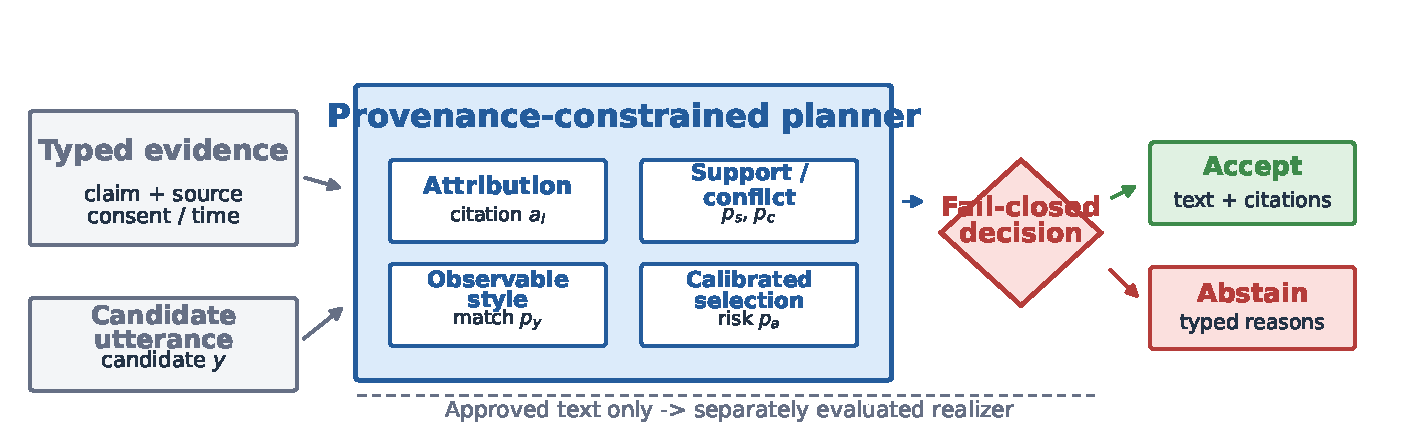
\includegraphics[width=.92\textwidth]{figures/method_overview.pdf}
  \caption{Language-only method overview.  Typed evidence and a candidate
  utterance are encoded separately; attribution, support, style, and conflict
  heads feed a calibrated fail-closed decision.  Downstream realization is an
  interface, not a result claimed by this paper.}
  \label{fig:method}
\end{figure*}

\section{Task Definition}

\subsection{Typed evidence}

For a target speaker $s$, the authorized evidence set is
$E_s=\{e_i\}_{i=1}^{n}$.  Each item is a tuple
\begin{equation}
 e_i=(x_i,t_i,r_i,\tau_i,c_i,q_i,u_i),
\end{equation}
where $x_i$ is text, $t_i$ is evidence type, $r_i$ is source identity,
$\tau_i$ is time period, $c_i$ is consent status, $q_i$ is stance
(support, contradiction, or uncertainty), and $u_i$ is source confidence.
Types distinguish direct messages and recorded transcripts from family
recollections, documented facts, and style observations.  The representation
does not imply that all sources have equal authority.

The most conservative executable policy accepts only a normalized exact match
to a consented first-party message or transcript.  This provides a non-neural
lower bound with maximal precision but low coverage.  Learned planning is
allowed to exceed this coverage only when claim annotations and citation
evaluation show that support is retained.

\subsection{Outputs and fail-closed semantics}

Given candidate $y$, the planner outputs support probability $p_s$, style-match
probability $p_y$, conflict probability $p_c$, a selectively trained score
$p_{sel}$ when all joint labels are available, and attribution scores $a_i$ for
every evidence item.  With thresholds selected
only on development speakers, synthesis is permitted iff
\begin{equation}
 p_a \geq \theta_a \land p_s \geq \theta_s \land
 p_c < \theta_c \land \exists i: a_i \geq \theta_e.
 \label{eq:decision}
\end{equation}
Otherwise the planner returns \textsc{abstain} and machine-readable reasons.
Here $p_a=p_{sel}\max_i a_i$ for jointly labelled episodes.  For style-only or
legacy checkpoints, $p_{sel}$ is replaced by the auditable product
$p_sp_y(1-p_c)$.  Independent support, conflict, and citation gates remain
mandatory, so a learned score cannot bypass a failed evidence gate.  A fluent
answer without an attributed evidence item cannot pass.

Accepted output remains synthetic.  Citation means that specified evidence
supports a claim under the annotation policy; it does not mean that the target
speaker authored the generated sentence.  Interfaces must preserve this
distinction in disclosure and audit records.

\section{Method}

\subsection{Sparse observable style}

We avoid treating Big Five prediction as a direct proxy for idiolect.  Instead,
the auditable style vector contains message and sentence length, length
variance, type--token ratio, function and discourse markers, punctuation,
questions and exclamations, politeness and uncertainty markers, first-person
rate, code switching, emoji rate, and lexical preferences.  Only consented,
non-disputed first-party records contribute to this vector.

For the executable baseline, token unigrams and local bigrams are mapped to a
signed hashing vector $v(x)\in\mathbb{R}^d$ and normalized.  A small feed-forward
encoder $g$ produces $h_x=g(v(x))$.  Evidence embeddings are mean pooled,
$h_E=n^{-1}\sum_i h_{x_i}$, and paired with candidate embedding $h_y$ as
\begin{equation}
 h_{E,y}=[h_E;h_y;|h_E-h_y|;h_E\odot h_y].
\end{equation}
The hashed bag-of-ngrams encoder is deliberately modest: it establishes a
reproducible CPU baseline and makes failures inspectable.  Our contextual
model uses a frozen MiniLM encoder followed by a trainable projection and the
same decision heads.  Encoder revision, sequence limit, and initialization
seed are stored in the checkpoint; frozen foundation weights are reloaded by
revision rather than duplicated.  Private memorial data are not sent to a
remote inference API.

Held-out authorship is used as a proxy task: evidence messages precede the
candidate chronologically, and negatives come only from another speaker in the
same split.  This tests whether style features identify a writer rather than
memorizing target-speaker IDs.  Topic leakage is measured through topic-matched
negative subsets, following the concern that author representations may encode
content rather than style \citep{wegmann-etal-2022-author}.

\subsection{Support, attribution, and conflict}

Rather than mean-pooling every source equally, the contextual model computes
candidate-conditioned evidence weights
\begin{equation}
 \alpha_i=\operatorname{softmax}_i(h_i^\top h_y/\sqrt{d}),\qquad
 h_E=\sum_i\alpha_i h_i.
\end{equation}
This attention is not itself a citation: the citation head below receives
direct supervision and is evaluated against evidence IDs.  An ablation restores
mean pooling.

The frozen observable-style features from the previous subsection are computed
separately for evidence and candidate.  Their vectors and absolute difference
are projected to $h_o$ and appended to $h_{E,y}$.  Removing $h_o$ tests whether
the neural encoder, rather than explicit linguistic features, accounts for a
gain.  Separate heads map $[h_{E,y};h_o]$ to support, style, conflict, and
selective logits.  The selective head is trained only when all joint labels are
present; missing axes remain masked rather than imputed.
Evidence attribution cannot be recovered from an aggregate head, so each item
is also paired with the candidate:
\begin{equation}
 \begin{split}
 h_{i,y}&=[h_i;h_y;|h_i-h_y|;h_i\odot h_y],\\
 a_i&=\sigma(w_e^\top h_{i,y}+b_e).
 \end{split}
\end{equation}
Acceptance combines the calibrated selective score with the maximum
evidence-attribution score.  The independent component gates in
Equation~\ref{eq:decision} keep the decision inspectable and fail closed.

Support and conflict require claim-level annotation.  Crucially, a held-out
message by the same writer supplies a style label but not a support label: the
speaker's earlier messages need not entail the later message.  Missing task
labels are masked rather than silently set to zero.  This prevents an easy but
invalid training shortcut.

For available labels, the objective is
\begin{equation}
 \begin{split}
 \mathcal{L}={}&\mathcal{L}_{style}+m_s\mathcal{L}_{support}
 +m_c\mathcal{L}_{conflict}\\
 &+m_e\mathcal{L}_{cite}+m_{joint}\mathcal{L}_{sel}.
 \end{split}
\end{equation}
where each component is binary cross entropy and $m$ indicates that the
corresponding annotation exists.  No cross-dataset pseudo-label is introduced
for a missing axis.

\begin{figure*}[t]
  \centering
  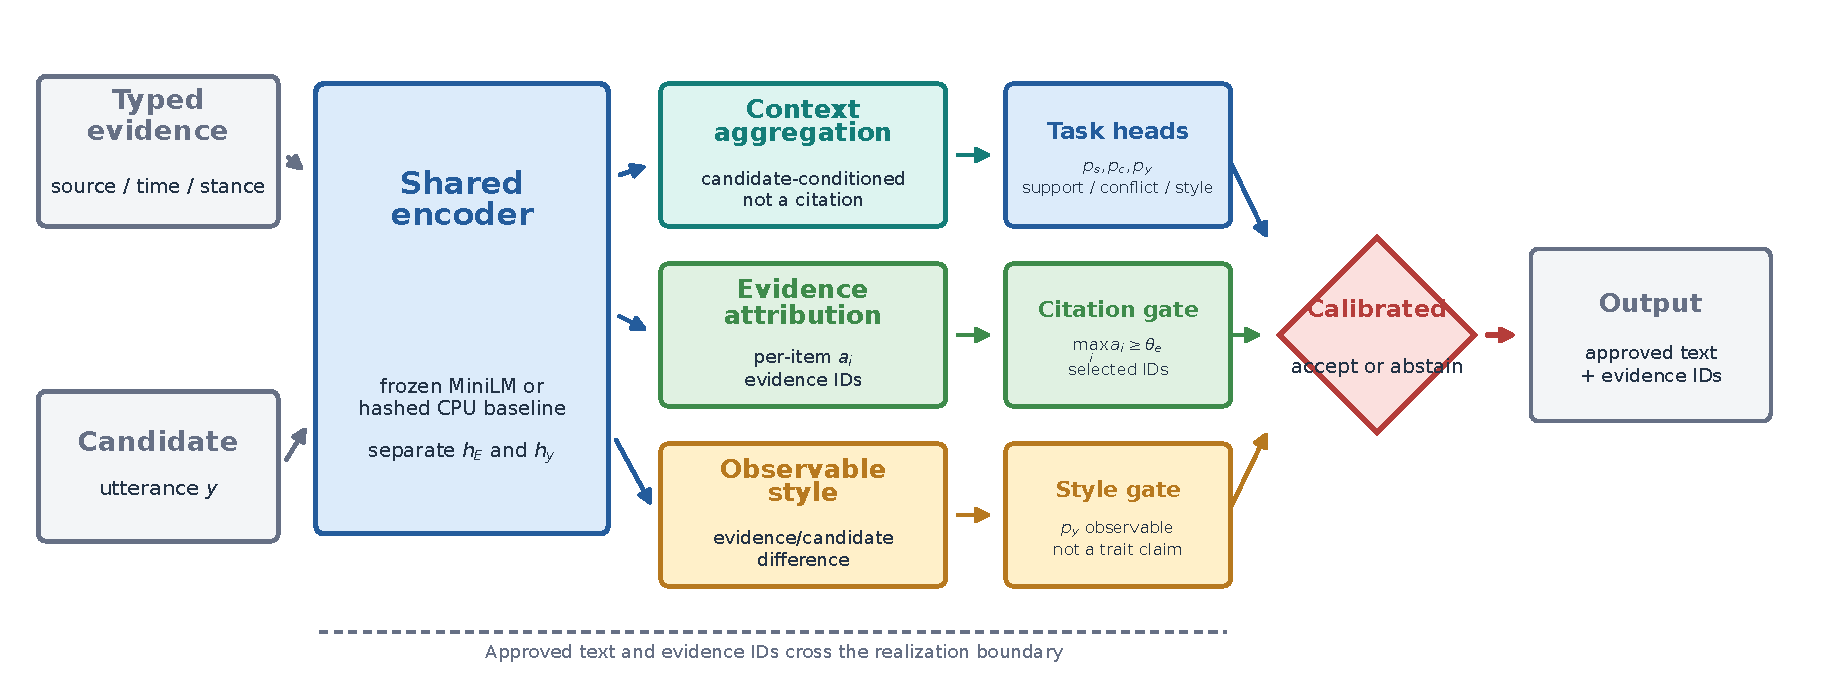
\includegraphics[width=.92\textwidth]{figures/planner_mechanism.pdf}
  \caption{Mechanism detail. Candidate-conditioned attention forms an aggregate
  context but is not treated as provenance. A separately supervised attribution
  head predicts evidence IDs, while support, conflict, and observable-style
  signals remain inspectable before calibrated selection.}
  \label{fig:planner-mechanism}
\end{figure*}

\subsection{Calibration and abstention}

Selective prediction is central rather than an auxiliary metric
\citep{xin-etal-2021-art,kamath-etal-2020-selective}.  Temperature or isotonic
calibration, decision thresholds, and the citation threshold are fit on
development speakers only.  We report expected calibration error (ECE),
coverage, selective risk, false acceptance, and false abstention.  A single
accuracy at $\theta=0.5$ is insufficient because the intended operating point
prioritizes avoiding unsupported accepted speech.

Conflicting sources are not averaged into a confident pseudo-consensus.  Any
gold contradiction must either be surfaced or trigger abstention.  We evaluate
conflict precision and recall, source-pair breakdowns, and a conflict
preservation score.  Recollection-only evidence cannot establish a first-party
quotation even if sources agree.

\subsection{Downstream realization boundary}

The planner emits an auditable approved-text record containing the selected
evidence IDs, decision reasons, and disclosure status.  A downstream speech
realizer may consume this record, but it must not bypass the planner or turn
style evidence into a first-person factual claim.  Voice cloning, acoustic
controls, reference-duration curves, and listening studies require a separate
evaluation; no acoustic result is used to support the language claims in this
paper.

\section{Public Proxy and Independent Labels}

The preferred dataset contains living speakers who explicitly consent to
  research use.  For public reproducibility, an openly licensed PersonaChat or
  ConvAI2-style export \citep{zhang2018personalizing} may be used as a
  \textsc{public-research}, text-only proxy;
it grants no permission to clone a participant's voice and is not a memorial
  source.  FEVER- and SciFact-style evidence data
  \citep{thorne2018fever,wadden2020fact} can evaluate support and conflict heads
  but cannot establish personal style.  Each record retains stable
speaker and conversation IDs, timestamp, consent scope, license identifier, and
source.  Private text is stored locally; release manifests contain hashes and
non-sensitive metadata.  The exact composite protocol and conversion script
are documented in \texttt{docs/research/PUBLIC\_DATASETS.md}.

\subsection{Independent compositional benchmark}

The principal controlled benchmark combines labels that were collected
independently of our system.  SNLI supplies human
\textsc{entailment}, \textsc{neutral}, and \textsc{contradiction} relations
\citep{bowman2015snli}; PersonaChat supplies a separate role-instance style
label.  We preserve SNLI's official splits, sample each relation equally, and
pair every sampled relation with one positive and one negative style episode.
This produces 12,000 training, 3,000 development, and 3,000 test episodes.

Each episode contains the annotated premise, three length-matched SNLI premise
distractors, and only the PersonaChat evidence supplied with that episode.
The gold premise position rotates deterministically, preventing a positional
shortcut.  A citation identifies the premise on which the annotated NLI
relation was judged; for neutral or contradictory hypotheses it does not mean
that the premise supports the hypothesis as true.  All policies receive this
same episode-local evidence budget.  SNLI is CC BY-SA 4.0 and PersonaChat is CC
BY 4.0; neither requires an approval workflow.  Source hashes, construction
seed, label mapping, and the final manifest fingerprint are frozen.

This composition supplies independent evidence, relation, style, and citation
targets at useful scale, but it is deliberately not described as naturally
generated personal speech.  A single SNLI premise is not a consent record, and
a PersonaChat role is not a stable living-speaker identity.

Speakers, not messages, are assigned to train, validation, and test.  The split
is produced by a seeded hash ranking and checked so no target or negative
candidate speaker crosses a split.  Retrieval indexes, prompts, calibration,
and model selection are also split-scoped.  With at least six speakers, each
holdout receives at least two speakers to support within-split negatives.

For each speaker, the chronologically last eligible message is a candidate and
earlier messages form evidence budgets $B\in\{1,2,5,10,25,\mathrm{all}\}$.
Positive style pairs use the same speaker; negative pairs use another speaker
within the same split.  In addition to the cyclic negative baseline, we build a
topic-matched condition by selecting a different role instance with maximal
token-Jaccard overlap using only split-local candidate text.  Full planner episodes additionally require atomic claim
support, contradiction, and evidence-attribution labels.  Annotators see source
type and time but not model predictions.  Ambiguous cases retain an
\textsc{uncertain} label rather than forced consensus.

\subsection{Annotation protocol}

Candidate utterances are segmented into minimal independently checkable claims.
Pure discourse markers receive a style-only tag.  For each remaining claim, two
annotators independently select zero or more evidence IDs and one relation:
\textsc{supported}, \textsc{contradicted}, \textsc{both},
\textsc{uncertain}, or \textsc{not-addressed}.  \textsc{Both} is retained when
authorized sources support incompatible values; it is not converted to a
majority label.  Annotators also mark exact quotation, close paraphrase, or
novel wording.

The guide distinguishes statement attribution from world truth.  A direct
message supports the claim that its author wrote the message, but not
automatically every proposition inside it.  A recollection can support
``source $r$ recalls phrase $p$,'' but cannot support ``speaker $s$ said $p$''
without first-party corroboration.  Time-sensitive claims must cite evidence
from the relevant period.

Agreement is reported separately for claim boundaries, evidence selection, and
relations.  Evidence selection uses set F1 and relation labels use nominal
Krippendorff's alpha.  Development disagreements refine the guide; test
disagreements are adjudicated under the frozen guide.  We report both
pre-adjudication agreement and adjudicated scores.  Annotators are never asked
to infer a clinical or psychological state.

\subsection{Data quality and exclusion gates}

Records are excluded before splitting when authorization or license fields are
missing, the speaker ID cannot be stabilized, text is machine generated, or a
timestamp required for chronological construction is unavailable.  Duplicate
and near-duplicate messages are grouped before splitting and cannot occur as
both evidence and held-out targets.  Forwarded or quoted spans are marked so
they do not become evidence of the account owner's style.

Language and script are recorded per message.  Code-switched messages remain
but are analyzed separately.  Minimum speaker and message counts are declared
before training.  If a language lacks the predeclared number of test speakers,
its results are descriptive and are not pooled into the principal endpoint.

\begin{figure*}[t]
  \centering
  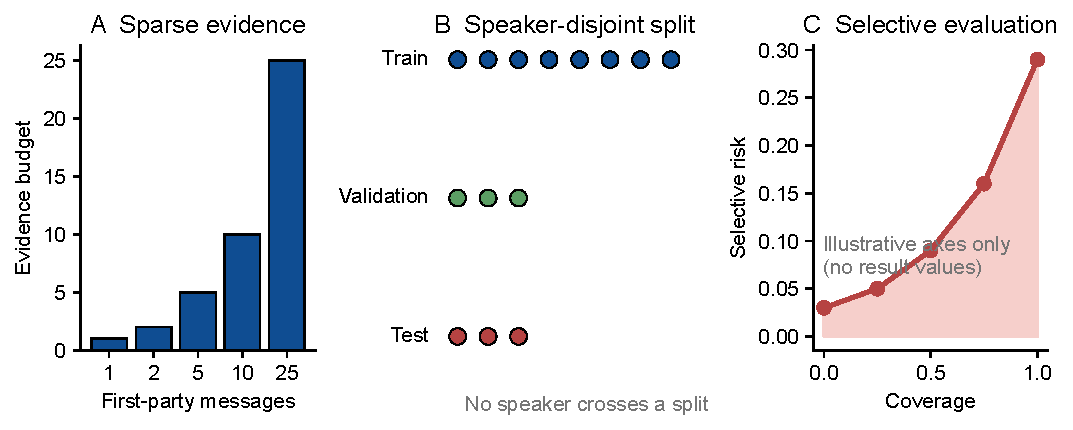
\includegraphics[width=.84\textwidth]{figures/experiment_protocol.pdf}
  \caption{Evaluation design.  Panel C illustrates the axes to be reported and
  contains no experimental result.  Final curves are generated only from a
  measured evaluation artifact.}
  \label{fig:protocol}
\end{figure*}

\section{Experimental Protocol}

\subsection{Language baselines and ablations}

The frozen baselines are: (1) neutral generic text with no target style;
(2) consented exact quotation; (3) retrieval-only nearest quotation; (4)
retrieval-augmented generation \citep{lewis2020rag} with citations and no style
component; and (5) the auditable hashed style planner.  Equal-budget contextual
baselines score only the evidence supplied in each episode: MiniLM and MPNet
top-1 retrieval, plus a top-2 selective RAG-style attribution policy whose
score threshold is fit on development data at a 90\% citation-precision floor.
Encoder names and exact revisions are stored in the artifact.  If a larger
language model is evaluated, its prompt, decoding
parameters, model revision, and any remote data retention must be reported.

Ablations remove provenance constraints, attribution supervision, conflict
handling, abstention, observable style features, and chronological evidence
selection one at a time.  We also compare first-party-only evidence against
recollection-enhanced retrieval.  The latter must never improve coverage by
mislabeling recalled wording as a quotation.

\subsection{Predeclared hypotheses}

H1 concerns coverage and risk.  Exact quotation should have the lowest
unsupported-acceptance risk but limited coverage; the selective planner should
improve coverage at a fixed citation-precision floor.  The claim fails if
coverage rises by accepting recollection-only paraphrases as first-party speech.

H2 concerns sparse style.  Held-out authorship and observable-style distance
should improve with evidence budget, with diminishing gains.  A gain that
vanishes under topic-matched negatives counts as topic exploitation.  H3
concerns conflict: explicit conflict supervision should improve contradiction
recall without an unacceptable coverage loss on agreed claims.

Each hypothesis has one principal contrast; other analyses are secondary.
Hyperparameters and thresholds are frozen after development.  We report all
seeds and never select a seed by test performance.  If a hypothesis fails, its
architectural claim is removed rather than rewritten around a favorable
secondary metric.

\subsection{Language metrics}

Citation precision and recall operate on evidence IDs; supported-claim coverage
operates on atomic claims.  Factual precision is reported at the claim level,
in the spirit of fine-grained evaluation \citep{min-etal-2023-factscore}, but
against the authorized evidence set rather than an open web corpus.  Conflict
precision, recall, and F1 test whether disputed material is surfaced.

Style is measured with held-out authorship accuracy, retrieval rank, and
normalized distance over the frozen observable feature schema.  We report both
cyclic and token-Jaccard topic-matched negative conditions.  Exact and
near-verbatim overlap detect
privacy memorization.  Calibration uses ECE and reliability plots
\citep{guo2017calibration}; selective behavior uses risk--coverage and error
rates at a preregistered low-risk operating point.

All confidence intervals bootstrap speakers, not messages.  Paired comparisons
use speaker-level aggregates, with effect sizes and confidence intervals.
Message-level tests would inflate the effective sample size because messages
from one writer are dependent.

\subsection{Language-only claim gates}

All principal gates in this paper are language gates.  Acoustic reference
duration, speaker similarity, emotion perception, and control leakage are
explicitly out of scope.

\begin{table*}[t]
\centering
\footnotesize
\begin{tabular}{p{1.7cm}p{4.0cm}p{4.0cm}p{4.5cm}}
\toprule
Layer & Primary question & Required metric & Failure that blocks a claim \\
\midrule
Evidence & Is accepted content attributable? & Citation precision/recall, claim coverage & Missing or wrong evidence ID \\
Conflict & Is disagreement preserved? & Conflict precision/recall/F1 & Contradiction collapsed to consensus \\
Selection & Does the system know when to stop? & ECE, risk--coverage, false acceptance & High-confidence unsupported acceptance \\
Style & Is style distinct from topic? & Authorship, style distance, topic controls & Topic-only discrimination \\
\bottomrule
\end{tabular}
\caption{Claim gates.  Passing one layer does not compensate for failure in
another.}
\label{tab:gates}
\end{table*}

\subsection{Compute and reproducibility}

The transparent baseline uses a signed hashed input.  The contextual model uses
frozen \texttt{all-MiniLM-L6-v2} representations, a 128-unit projection, and a
96-token limit.  The reported PersonaChat run uses one epoch and batch size 128;
the matched compositional proxy uses a fixed maximum of 12 epochs and batch
size 32, with the selected epoch recorded in each checkpoint.  Both use AdamW
and gradient clipping at 1.0. Seeds,
dataset fingerprints, schema version, epoch, threshold, and metrics are stored
  with planner checkpoints.  This path is designed to run on commodity
  hardware.  Any downstream realizer must record its own hardware, model, and
  decoder revisions rather than mixing those measurements into this paper.

\subsection{Model selection and statistics}

Model selection is lexicographic.  Configurations must first satisfy a minimum
citation precision and maximum false-acceptance rate.  Among feasible models we
maximize coverage; style accuracy breaks remaining ties.  This prevents a
weighted average from exchanging a major safety regression for a small style
gain.  Thresholds may differ by evidence type but not by test speaker.

Paired comparisons use per-speaker differences and percentile bootstrap
intervals over speakers.  Binary outcomes also receive a paired permutation
test at speaker level.  Secondary contrasts use the Holm correction.  We report
effect sizes and practical margins rather than treating $p<.05$ as evidence of
equivalence.

Calibration is assessed globally and by evidence budget, language, and source
composition.  Because ECE depends on binning, equal-width bins are predeclared;
we also report Brier score and reliability diagrams.  Risk--coverage curves use
every unique acceptance threshold.  Their area is a summary, not a replacement
for the preregistered operating point.

\section{Results and Submission Gate}

Table~\ref{tab:results} reports the completed public role-instance style proxy
under both the original cyclic-negative condition and a harder topic-matched
condition.  Historical JSON files, UI demonstration values, untrained adapters,
and synthetic curves are excluded.
PersonaChat measures whether a candidate reply
matches the assigned dialogue role given that role's persona statements; it
does not measure a stable natural person, memorial fidelity, factual support,
or voice identity.

\begin{table*}[t]
\centering
\scriptsize
\begin{tabular}{llcc}
\toprule
Condition & Model & Seeds & Acc. / ECE \\
\midrule
Cyclic & Hash & 1 & 60.90 [59.25, 62.58] / 3.48 \\
Cyclic & MiniLM & 3 & $69.17\pm0.58$ / 3.07 \\
Topic & Hash & 1 & 62.53 [60.72, 64.28] / 7.06 \\
Topic & MiniLM & 3 & $65.03\pm0.03$ / 4.44 \\
\bottomrule
\end{tabular}
\caption{Measured PersonaChat role-instance style attribution (percent; ECE is
reported in percentage points).  Accuracy intervals for one-seed rows are
speaker bootstrap intervals; multi-seed rows report mean $\pm$ sample standard
deviation and average ECE.  Topic-matched negatives reduce MiniLM accuracy by
4.14 points relative to cyclic negatives, while preserving a 2.50-point
advantage over the matched hash baseline.}
\label{tab:results}
\end{table*}

\begin{figure}[t]
  \centering
  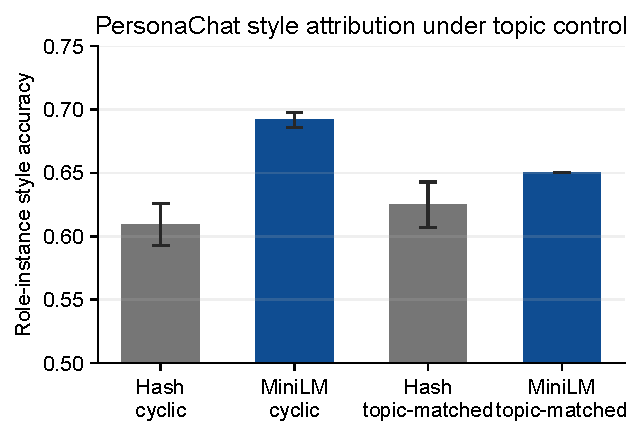
\includegraphics[width=.82\columnwidth]{figures/planner_comparison.pdf}
\caption{Measured public proxy comparison under cyclic and topic-matched
negatives.  Error bars show a bootstrap interval for the one-seed hash runs and
across-seed standard deviation for MiniLM; they therefore answer different
uncertainty questions.}
  \label{fig:planner-results}
\end{figure}

The full planner's principal endpoint is citation precision at a declared
operating point, not the largest raw coverage.  Table~\ref{tab:joint-results}
reports the frozen SNLI--PersonaChat compositional test over three seeds.  A
frozen semantic citation prior plus a learned bounded residual raises citation
recall while a two-layer selective head ranks jointly valid cases.  Selection
and component-gate thresholds are separate parameters; an implementation audit
found and corrected an earlier contract that accidentally reused the selection
threshold for every component gate.

The planner reaches $90.39\%\pm0.33$ micro citation precision,
$74.03\%\pm0.87$ recall, and $68.70\%\pm0.77$ conflict F1.  Positive-case
coverage rises from zero in the legacy SciFact diagnostic to
$3.73\%\pm4.24$ here, but remains too low.  More importantly, a maximum 5\%
development false-acceptance constraint yields $23.62\%\pm3.17$ on test.  H1
therefore fails: the development operating point is not a transferable safety
guarantee.  No seed is selected post hoc.

\begin{table*}[t]
\centering
\scriptsize
\setlength{\tabcolsep}{3.5pt}
\begin{tabular}{lccccccc}
\toprule
Model & Style & Cite P & Cite R & Conflict & Pos. cov. & False acc. & ECE \\
\midrule
Selective planner & $72.27\pm0.44$ & $90.39\pm0.33$ & $74.03\pm0.87$ & $68.70\pm0.77$ & $3.73\pm4.24$ & $23.62\pm3.17$ & $15.21\pm1.89$ \\
\bottomrule
\end{tabular}
\caption{Measured independent-label compositional test (percent; mean $\pm$
sample standard deviation over three seeds).  False acceptance is the fraction
of accepted cases whose joint target is negative.  The development ceiling was
5\%; its test violation is a failed hypothesis, not a safety claim.}
\label{tab:joint-results}
\end{table*}

Table~\ref{tab:contextual} and Figure~\ref{fig:contextual} compare attribution
under exactly the same episode-local evidence.  Top-1 retrieval is a strong
baseline.  Selective RAG-2 exchanges recall for precision; only MiniLM RAG-2
meets the 90\% test precision level.  The planner has comparable precision but
lower recall because its citation cutoff is coupled to a broader joint task.
At the 1,500 SNLI source-group level, its recall difference from MiniLM RAG-2
is $-0.73$ points (paired bootstrap 95\% CI $[-1.87,0.43]$; Holm-adjusted
sign-flip $p=.210$), so we do not detect a difference for that contrast.  It is
significantly lower than both top-1 policies and MPNet RAG-2.

\begin{table}[t]
\centering
\scriptsize
\begin{tabular}{lcc}
\toprule
Equal-budget policy & Cite P & Cite R \\
\midrule
MiniLM top-1 & 88.73 & 88.73 \\
MiniLM selective RAG-2 & 91.51 & 74.77 \\
MPNet top-1 & 89.63 & 89.63 \\
MPNet selective RAG-2 & 89.48 & 78.00 \\
Planner (3 seeds) & $90.39\pm0.33$ & $74.03\pm0.87$ \\
\bottomrule
\end{tabular}
\caption{Micro citation scores on the SNLI composition test (percent).  RAG-2
thresholds are fit only on development data; no method retrieves evidence
outside the episode.}
\label{tab:contextual}
\end{table}

\begin{figure}[t]
  \centering
  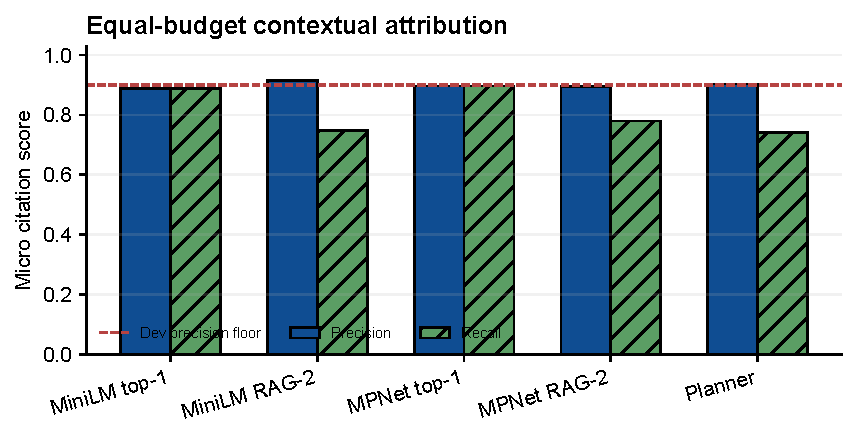
\includegraphics[width=\columnwidth]{figures/contextual_baselines.pdf}
  \caption{Measured equal-budget contextual baselines.  The dashed line is the
  predeclared 90\% development precision floor, not a test guarantee.}
  \label{fig:contextual}
\end{figure}

\begin{figure*}[t]
  \centering
  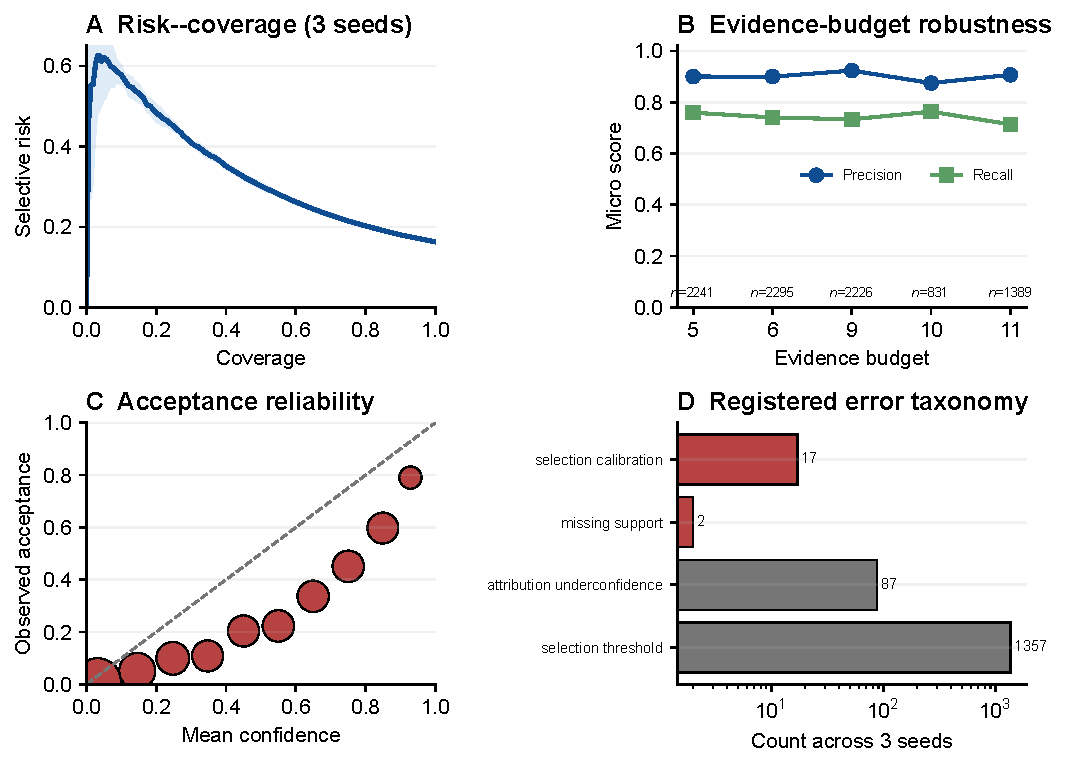
\includegraphics[width=.84\textwidth]{figures/joint_diagnostics.pdf}
  \caption{Measured SNLI-composition diagnostics.  Shading in A is one sample
  standard deviation over three seeds.  B excludes evidence-budget cells with
  fewer than 100 pooled observations and prints each retained $n$.  Bubble area
  in C reflects bin count.  D uses a log count axis; red denotes false
  acceptance and gray false abstention.}
  \label{fig:joint-diagnostics}
\end{figure*}

\subsection{Evidence budget and provenance ablation}

The frozen test rows expose a useful distinction between adding evidence and
removing the provenance contract.  Figure~\ref{fig:budget-tradeoff} pools the
three registered seeds and groups by the actually observed episode budgets
($5,6,9,10,11$; the two larger cells are retained but not interpreted because
they contain fewer than 20 rows).  The constrained planner accepts only a few
percent of positive cases, but its acceptance error is generally lower than a
provenance-free replay.  The replay uses the fixed score
$p_s p_y$ and a threshold of $0.5$; it has no citation, conflict, or evidence
type gate and is not tuned on the test split.  Its positive coverage is roughly
$46$--$54\%$, accompanied by $34$--$48\%$ false acceptance.  This is the
operational value of typed evidence and conflict preservation: they reduce the
set of fluent but unauthorized candidates, even though the present calibration
does not achieve the desired coverage.

\begin{figure}[t]
  \centering
  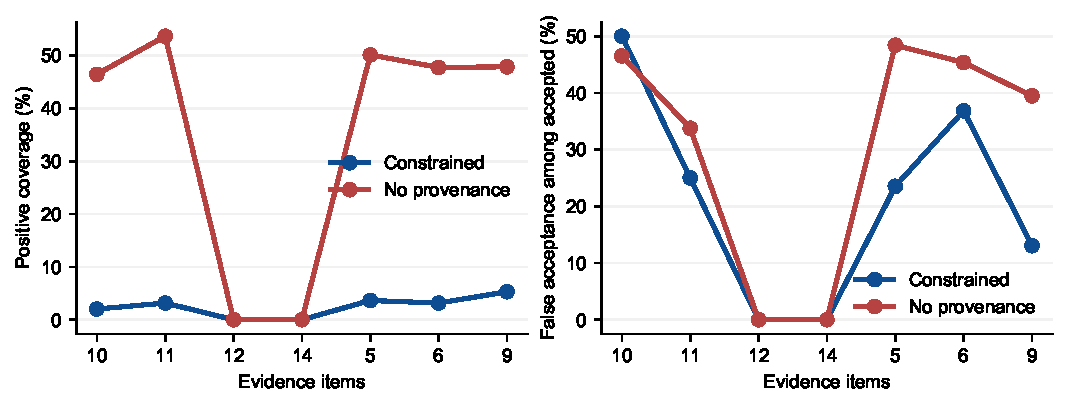
\includegraphics[width=.84\columnwidth]{figures/evidence_budget_tradeoff.pdf}
  \caption{Evidence-budget replay on the untouched test rows.  The constrained
  decision retains provenance and conflict gates; the no-provenance score is
  the fixed $p_s p_y$ replay.  Budgets are the observed cells, not an invented
  regular grid.}
\label{fig:budget-tradeoff}
\end{figure}

The requested $\{1,2,3,5,10\}$ evidence grid is only partially observable in
the released predictions.  Table~\ref{tab:requested-budget} reports the two
requested cells that are genuinely present; the 1/2/3 cells are marked as
unavailable because truncating a 5--11-item prediction would not reproduce a
planner inference.  This distinction matters: evidence budget is an input to
retrieval, attribution, and conflict scoring, not merely a post-hoc mask.

\begin{table}[t]
\centering
\scriptsize
\setlength{\tabcolsep}{2pt}
\begin{tabular}{lrrrrr}
\toprule
Budget & Cite P & Cite R & Pos. cov. & False acc. & Status \\
\midrule
1 & -- & -- & -- & -- & not run \\
2 & -- & -- & -- & -- & not run \\
3 & -- & -- & -- & -- & not run \\
5 & 94.12 & 75.90 & 3.64 & 23.53 & measured \\
10 & 100.00 & 76.29 & 2.02 & 50.00 & measured \\
\bottomrule
\end{tabular}
\caption{Requested evidence-budget grid on the frozen test snapshot. Cite P
is accepted-case citation precision; coverage is positive-case coverage and
false acceptance is the fraction of accepted cases with a negative joint
target. Dashes are deliberate: no low-budget planner re-evaluation is
available.}
\label{tab:requested-budget}
\end{table}

The failure ledger makes the negative result more specific.  The source audit
contains 17 false acceptances tagged as selection-calibration errors and two
as missing support, alongside 1,357 false abstentions at the selection
threshold and 87 attribution-underconfidence cases.  A secondary replay
labels the 17 negative-style accepts as style-overfit and reproduces the two
missing-support rows across seeds; no accepted contradictory row appears in
this benchmark.  That zero is a construction limitation, not evidence that
conflict handling is solved: the composition supplies few adversarial
contradictions and should be extended with naturally disputed, source-typed
episodes before any deployment claim.

\begin{table}[t]
\centering
\scriptsize
\begin{tabular}{lrrrr}
\toprule
Budget & Sel. abst. & Attr. abst. & Miss. sup. & Calib. FA \\
\midrule
5  & 14.55\% & 0.80\% & 0.04\% & 0.13\% \\
6  & 15.69\% & 0.39\% & 0.00\% & 0.31\% \\
9  & 14.60\% & 1.48\% & 0.00\% & 0.13\% \\
10 & 11.43\% & 0.24\% & 0.12\% & 0.12\% \\
11 & 18.07\% & 1.80\% & 0.00\% & 0.22\% \\
\bottomrule
\end{tabular}
\caption{Failure rates normalized by all pooled frozen rows in each observed
evidence-budget cell.  Selection-threshold false abstention dominates every
cell; the accepted-error rates remain sparse but do not vanish with more
evidence.}
\label{tab:failure-by-budget}
\end{table}

\subsection{Cross-domain structural audit}

To test whether the evidence-budget interface is tied to PersonaChat's
conversation format, we ran a separate deterministic audit on the official
DailyDialog test archive \citep{li2017dailydialog} (958 eligible dialogues and one fixed target turn per
dialogue).  This auxiliary audit does not rerun the learned
planner and does not introduce entailment annotations.  A prior turn is
defined as lexical evidence when it shares a non-stopword with the target;
the definition is deliberately weak and is reported as such.  The result is a
useful stress test of evidence availability and citation dilution, not a
cross-dataset safety claim.

\begin{table}[t]
\centering
\scriptsize
\begin{tabular}{lrrrr}
\toprule
Budget & Eligible & Support cov. & Top-1 P & Top-1 R \\
\midrule
1 & 276 & 28.81\% & 100.00\% & 100.00\% \\
2 & 418 & 43.63\% & 87.32\% & 100.00\% \\
3 & 468 & 48.85\% & 80.02\% & 100.00\% \\
5 & 534 & 55.74\% & 70.84\% & 100.00\% \\
\bottomrule
\end{tabular}
\caption{DailyDialog lexical-evidence audit on the official test split.  The
support label is token overlap rather than human entailment; top-1 recall is
therefore an availability diagnostic, not factual citation recall.}
\label{tab:dailydialog}
\end{table}

The monotone increase in lexical support coverage is accompanied by lower
top-1 precision as additional turns create more plausible sources.  This
direction matches the provenance concern exposed by the SNLI composition:
more evidence can increase recall while making source attribution less
selective.  Because DailyDialog has no speaker authorization or claim-level
support labels in this release, we do not pool its numbers with the principal
endpoint.

\begin{figure}[t]
  \centering
  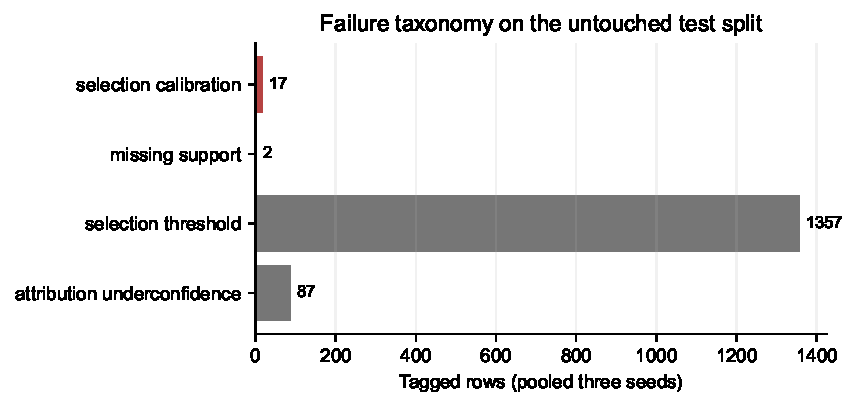
\includegraphics[width=.84\columnwidth]{figures/failure_taxonomy.pdf}
  \caption{Registered failure tags pooled over three seeds.  Selection
  thresholding dominates false abstention; the accepted-error mass is small but
  concentrated in calibration/style-overfit cases.}
  \label{fig:failure-taxonomy}
\end{figure}

Table~\ref{tab:ablations} preserves the declared architectural ablations on
the earlier SciFact--PersonaChat transfer diagnostic.  The single-seed rows use the earlier v5
checkpoints loaded through the explicit v7 migration path; they are included
as diagnostics, not as additional seed evidence.  Removing observable style
features reduces style attribution, while removing attention changes the
trade-off rather than establishing a universal win.  The no-selective row
uses the registered legacy support--style--conflict product with its own
development calibration.

\begin{table}[t]
\centering
\scriptsize
\setlength{\tabcolsep}{2.5pt}
\begin{tabular}{lccccc}
\toprule
Ablation & Style & Cite P & Cite R & Conflict F1 & ECE \\
\midrule
Full (3 seeds) & 67.64 & 88.63 & 35.33 & 30.41 & 4.01 \\
No attention & 68.88 & 94.35 & 27.99 & 6.94 & 3.23 \\
No style & 63.56 & 94.96 & 27.03 & 1.41 & 1.44 \\
No selective & 66.49 & 94.31 & 27.75 & 29.87 & 3.40 \\
\bottomrule
\end{tabular}
\caption{Legacy single-seed ablations on the SciFact compositional test split
(percent; ECE in percentage points).  Full-row values are the three-seed
means; ablations are measured diagnostics with separate development
calibration and are not selected on test performance.}
\label{tab:ablations}
\end{table}

\section{Error Analysis Protocol}

Every false acceptance receives one primary and any number of secondary tags:
missing support, wrong source, wrong period, unresolved contradiction,
quotation inflation, topic--style confusion, calibration error, or policy
bypass.  False abstentions are divided into retrieval failure, attribution
under-confidence, over-sensitive conflict detection, and style
under-confidence.  Counts and rates are reported by evidence budget and source
composition.

Qualitative examples contain synthetic or separately release-authorized text,
never private test messages.  Each shows typed evidence IDs, gold and predicted
citations, probabilities, decision reasons, and the minimal change that flips
the decision.  Failures are included.  Counterfactual examples exchange topic
while approximately holding function-word and punctuation profiles fixed, or
exchange style while holding topic fixed, probing whether the style head uses
content shortcuts.

Audio errors and acoustic leakage are outside this paper's error analysis.
Across three SNLI-composition seeds, the registered taxonomy contains 1,357
positive cases stopped by the selection threshold and 87 stopped by
attribution under-confidence.  The 19 false acceptances comprise 17 selection
calibration errors and two missing-support cases.  These counts explain why
increasing coverage by simply lowering the threshold is not justified.
The released ID-only artifact \texttt{snli\_error\_analysis.json} contains
the same tags by evidence budget and capped episode examples; it contains no
private message text.

\section{Reproducibility Artifacts}

The implementation writes immutable JSONL episodes, a manifest fingerprint,
planner checkpoints, and machine-readable evaluation rows.  A checkpoint
contains its schema, dimensions, seed, epoch, threshold, data fingerprint, and
measured development metrics.  Loading may require an expected fingerprint,
preventing accidental evaluation against a different manifest with the same
filename.
The contextual-baseline artifact records frozen encoder revisions, local-only
loading, validation and test fingerprints, top-$k$, calibrated threshold, and
the equal-evidence-budget policy.  The three-seed aggregate exposes positive
coverage directly rather than requiring it to be inferred from abstention.
The paired-analysis artifact averages the two style variants within each of
1,500 SNLI source groups, then records bootstrap intervals, seeded sign-flip
tests, and Holm-adjusted $p$ values.

Conceptual figures are deterministic.  Result figures reject inputs not marked
as measured evaluation runs and fail when rows are absent.  Code, frozen
predictions, and SHA-256 manifests for this version are available in the
\href{https://github.com/FinalSunFlower/PersonaVoice/tree/paper-supplement-v1.0}{paper-supplement-v1.0 GitHub snapshot}.
The exact artifact snapshot corresponding to this preprint is tagged
\texttt{paper-language-v1.0}.  The release separates code, consent-safe
manifests, model cards, and any restricted data-access process; no private
messages or raw audio are redistributed.

\section{Ethics, Governance, and Threat Model}

The system requires an explicit authorization basis, declared purpose,
synthetic-content disclosure, and a revocation channel before synthesis.  The
server validates these fields before model loading and stores hashes rather
than raw submitted text or audio in its audit record.  Memorial-mode content
also requires a server-validated plan; client-provided ``allowed'' flags are
ignored.

Threats include impersonation, fraud, harassment, reputational harm, fabricated
political or financial statements, family conflict, privacy leakage, and
emotional dependency.  Voice resemblance amplifies these risks.  A research
prototype therefore uses living-speaker proxy data, visible disclosure,
fail-closed consent, exact-quotation fallback, rate limiting at deployment, and
revocation.  Release should omit private training data and unrestricted
identity checkpoints.

Consent from one relative does not settle ownership, privacy, publicity,
copyright, or moral rights.  Applicable law varies by jurisdiction.  A future
study with bereaved people would require prospective ethics review, a distress
and withdrawal protocol, data-protection review, and careful eligibility rules;
approval cannot be obtained retrospectively.  No psychological benefit is
claimed by the present technical work.

\section{Related Work}

\paragraph{Style and personality.}
Language correlates with personality labels at population scale
\citep{mairesse2007linguistic,schwartz2013personality}, but this does not license
recovering an individual's ``true personality'' from sparse family-selected
  text.  Authorship attribution has a long stylometric tradition
  \citep{stamatatos2009survey}, while content-independent representations remain
  vulnerable to topic effects \citep{wegmann-etal-2022-author}. Persona dialogue
  models condition generation on speaker descriptions or histories
  \citep{li2016persona,zhang2018personalizing}; our question is instead whether a
  candidate can be authorized by sparse typed evidence without converting
  persona descriptions into factual claims.

\paragraph{Grounding and selection.}
Citation-aware generation measures whether claims are attributable
\citep{gao-etal-2023-enabling}, while atomic factuality metrics expose errors
hidden by document-level scores \citep{min-etal-2023-factscore}.  Selective NLP
adds the ability to abstain under uncertainty
\citep{xin-etal-2021-art,kamath-etal-2020-selective}.  Our setting combines these
  requirements with typed private evidence and explicit source disagreement.
  Fact-verification benchmarks provide support and contradiction supervision
  \citep{thorne2018fever,wadden2020fact}, but their labels do not encode speaker
  consent, source authority, personal style, or authorization to speak in the
  first person. Retrieval-augmented and self-critical generation
  \citep{lewis2020rag,asai2024selfrag,manakul2023selfcheckgpt} likewise require an
  explicit evidence contract before use in this setting.

\paragraph{Downstream realization.}
Zero-shot voice generation can make unsupported language more persuasive
\citep{chen-etal-2025-f5,peng-etal-2024-voicecraft}.  We therefore expose a
fail-closed approved-text boundary, but acoustic modeling and controllability
are not contributions of this paper.

\section{Limitations}

The hashed encoder is a transparent baseline, not a competitive contextual
model.  Speaker-disjoint proxy data cannot reproduce posthumous consent
ambiguity, archival degradation, family dynamics, or grief.  First-party text
may be too sparse to identify stable style; uncertainty should then increase
rather than be filled by relatives' impressions.  Observable style features
are language- and culture-dependent, and markers require validation beyond
English and Mandarin.

Evidence attribution does not prove truth.  A first-party message can be false,
sarcastic, outdated, quoted from someone else, or outside its consent scope.
Atomic claim annotation is costly and may disagree.  Calibration can shift
across domains, languages, source mixtures, and evidence budgets.  It does
shift here: a development false-acceptance ceiling of 5\% becomes
$23.62\%\pm3.17$ on the independent test split.  The current method is
therefore unsuitable for a deployment claim even though citation retrieval is
strong.

The measured style comparison uses three contextual-model seeds and one hash
seed in each negative policy.  PersonaChat roles remain constructed proxies,
and the topic-matched policy controls lexical overlap rather than establishing
causal topic independence; it therefore motivates, but does not replace,
jointly annotated speaker-disjoint data.
SNLI relations and PersonaChat style labels were independently collected, but
their composition is programmatic.  It cannot measure natural candidate
generation, pragmatic implicature, long-document retrieval, consent, or a
stable person's style.  Strong top-1 retrieval also shows that the benchmark's
attribution component remains substantially semantic and should not be used to
claim broad RAG superiority.
Finally, an accepted plan can still be harmful.  Technical controls cannot
resolve who has moral authority to represent a deceased person, and double
blind review does not remove these societal questions.  Deployment requires
jurisdiction-specific review and ongoing revocation, monitoring, and incident
response beyond this research prototype.

\section{Conclusion}

Memorial voice generation should not begin by asking how convincingly a system
can imitate a voice.  It should first ask what evidence authorizes a candidate
utterance, what is merely stylistic resemblance, where sources disagree, and
when the system must stop.  We provide an executable formulation of this NLP
problem, a selective evidence-level planner, and a speaker-disjoint proxy
protocol and an independently labelled compositional benchmark.  The planner
improves citation and conflict measurements, while equal-budget contextual
retrieval remains highly competitive.  The selective-risk hypothesis fails
under split shift, so the present result supports benchmark and diagnostic
claims, not safe deployment.  The system is not a claim of reconstructing a
person, and it makes no acoustic contribution.

\bibliography{personavoice}
\bibliographystyle{tacl-style/acl_natbib}

\end{document}
